%%%%%%%%%%%%%%%%%%%%%%%%%%%%%%%%%%%%%
\chapter{Short term quantum computing}
\label{Shortqcomp}

\epigraph{\textit{Let's put a nice quote here! A Quantum supremacy quote?}}{Andres} % a Q supreacy quote

In this section we aim to give a comprehensive overview of quantum computing platforms which are currently available and discuss the near-term advantages that these platforms can bring.

%%%%%%%%%%%%%%%%%%%%%%%%%%%%%%%%%%%%%%%%%%%%%%%%%%%%%%%%%%
%%%%%%%%%%%%%%%%%%%%%%%%%%%%%%%%%%%%%%%%%%%%%%%%%%%%%%%%%%
\section{Adiabatic quantum computing \& quantum annealers}
%%%%%%%%%%%%%%%%%%%%%%%%%%%%%%%%%%%%%%%%%%%%%%%%%%%%%%%%%%
%%%%%%%%%%%%%%%%%%%%%%%%%%%%%%%%%%%%%%%%%%%%%%%%%%%%%%%%%%

As the universal computer is hard to achieve in the short term requiring high quality and scalability of the qubits, the technology making use of existing qubits were proposed as the intermediate steps. One of them is quantum annealing. Annealing is a process to search for the minimum energy of the state. Classically this is done by the thermal annealing changing the temperature adiabatically. Quantum annealing is expected to be implemented more efficiently with the assistance of entanglement and tunneling as showed in \autoref{fig:Tunnelling}.\\
 
 Released by D-Wave Systems Inc. in 2017, state of the art quantum annealing computer D-Wave 2000Q has 2048 superconducting qubits connected with entanglement.  This is greatly improved  from the first prototype with 128 qubits. it can solve certain type of problems more efficiently than the classical computer. i.e. NP hard optimisation problems such as coloring problem.\\
  D-wave has its own software stack:
\begin{itemize}
    \item \textbf{D-Wave Ocean}- D-Wave toolkits to help solve problems on D-Wave system.
     \item \textbf{qbsolv}- Open source hybrid optimization solver which can partition the Quadratic unconstrained binary optimization (QUBO) which is run either on tabu classical solver or D-Wave system. By default classical solver is used. To use D-Wave machine, separate arrangement should be made.
    \item \textbf{QPU}- Quantum processing unit. API key is needed to run the program on the quantum computer.
 \end{itemize}
Alternatively, 1Qbit has developed the 1QBIT QUANTUM-READY™ software development kit targetting on hardware independent language. Currently it can use local classical solver or interface to D-Wave system with API key provided.
I will introduce the 1QBIT QUANTUM-READY™ SDK in this section, as the example of the language used as the interface to D-Wave machine. Currently only online Jupyter Notebook version is available on \url{http://qdk.1qbit.com/}.
By default classical solver is used. To use D-Wave machine, separate arrangement should be made.\\
Quantum annealing computer can be programmed to solve Quadratic unconstrained binary optimization (QUBO) problem. Given the coefficients $h_i$ and $J_{ij}$, QUBO problems are such that to determine the minimum value of
\begin{equation}
C=\sum_{i=1}^{N} h_iq_i+\sum_{i<j}^{N} J_{ij}q_iq_j\\\\\ q_i\in\{-1,1\}
\end{equation}
To have a better idea of this, I will borrow the example of the light switching game from \href{https://www.dwavesys.com/tutorials/background-reading-series/quantum-computing-primer}{D-Wave website}. Imagine there are several lights with  certain bias marked for each of them  and certain weight assigned between every two of them. For each switch, "ON" scores 1 point and "OFF" scores -1 point. The total score is the sum of the bias multiplied by the light configuration score. Additional score contribution exists from the weights multiplied by the two fold light configuration.  The goal is to set the light configuration such that the total score is minimum. If we have positive bias to all of the lights, it is easy to know such configuration is setting all the light "OFF". However it can be notoriously complicating to take the weights between the lights into account.\\
\begin{figure}[h!]
    \centering
    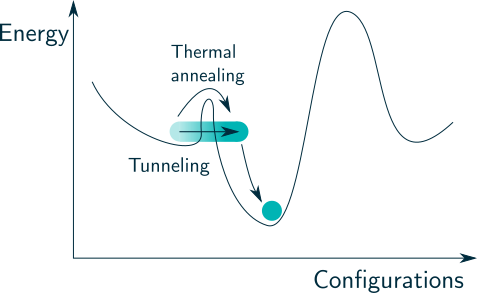
\includegraphics{figures/Tunneling.png}
    \caption{Caption}
    \label{fig:Tunnelling}
\end{figure}

\begin{tcolorbox}[standard jigsaw,
    opacityback=0,  % this works only in combination with the key "standard jigsaw"
    boxrule=0.5pt,label={example1}]
    {\bf Example 1}
    \tcbline
Solve the light configuration problem with two lights involved. The bias are set to be -1 for both lights and the weight assigned between them is 2 \\
i.e. Get the configuration to minimize the quadratic polynomial $-x_0-x_1+2x_0x_1$  
\end{tcolorbox}
\begin{lstlisting}[language=python]
from qdk import* 
# Create a quadratic polynmial  -x_0-x_1+2x_0x_1  
builder = QuadraticBinaryPolynomialBuilder() 
builder.add_term(-1.0, 0, 0) 
builder.add_term(-1.0, 1, 1) 
builder.add_term(2.0, 1, 0)  
quad_poly = builder.build_polynomial() 
# Create a local solver  
dwave_local_solver = DWaveSolver() 
# Get configuration of minimum energy solution 
solution_list = dwave_local_solver.minimize(quad_poly) 
print solution_list.solution_count 
sol=solution_list.peek_minimum_energy_solution() 
print sol 
\end{lstlisting}

Vertex coloring problem is probably one of the most popular NP problems. Given the graph G(V, E) with the set of vertices V and the set of edges E, it is to determine the coloring configuration of the vertices for which no adjacent two nodes (the nodes connected with edge) have the same color. \\ 
Mathematically it is the same as finding the minimum value for:
\begin{equation}
H = \sum_{n=0}^{N-1}(1-\sum_{k=0}^{K-1}x_{n,k})^2 + \sum_{(u,v)\in E}\sum_{k=0}^{K-1}x_{u,k}x_{v,k}
\end{equation}
$x_{n,k}$ with node n and color k is 1 only if the node n has color k, 0 otherwise. N is the total number of nodes and K is total number of the color used. The first term is the restriction that each node can only have one color. The second term is the restriction that the adjacent nodes have different color.  As only one dimensional QUBO problem can be solved, the equation (2) should be reduced to one dimension by reordering the index $n,k \rightarrow nK+k$. 
\begin{tcolorbox}[standard jigsaw,
    opacityback=0,  % this works only in combination with the key "standard jigsaw"
    boxrule=0.5pt,label={example1}]
    {\bf Example 2}
    \tcbline 
  Vertex  coloring problem for configuration showed in (a)
    \end{tcolorbox}
   
\begin{lstlisting}[language=python, caption={code adapted from KColoring.ipynb on   \url{ http://qdk.1qbit.com/}   }, label={code}]
import networkx as nx 
import matplotlib.pyplot as plt 
# Set the graph configuration by setting nodes and neighbours 
node=[0,1,2,3,4] 
neighbour=[(0,4),(1,2),(1,3),(1,4)] 
# Draw the graph configuration 
g=nx.Graph() 
g.add_nodes_from(node) 
g.add_edges_from(neighbour) 
pos = nx.spring_layout(g) 
nx.draw(g, pos=pos, with_labels=True) 
plt.show() 
# Turn the two dimension index to one dimension
def ind2to1(i, j, r):  
 return i * r + j  
pallete = {0: 'r', 1: 'c', 2:'m', 3:'y'} 
def get_color(i, sol, r): 
 z = ind2to1(i, 0, r) 
 ctr = 0 
 for ctr in range(r): 
  if sol[z + ctr]: 
   break 
 return pallete[ctr] 
# Construct the quadratic equation (3.2) with one dimension index
from qdk.binary_polynomial import * 
from qdk.common_solver_interface import * 
builder = QuadraticBinaryPolynomialBuilder() 
qubo = builder.build_polynomial() 
N = 5 
K = 4
for n in range(N): 
 builder.add_constant_term(1) 
for k in range(K): 
 builder.add_term(-1, ind2to1(n,k,K)) 
l=builder.build_polynomial() 
builder.power(2) 
t = builder.build_polynomial() 
qubo.sum(t) 
builder.reset() 
for (u,v) in g.edges(): 
 for k in range(K):  
  builder.add_term(1, ind2to1(u,k,K), ind2to1(v,k,K)) 
qubo.sum(builder.build_polynomial()) 
print qubo 
# Get the minimum energy solution by taking 300 samples
solver = DWaveSolver() 
solver.solver.num_reads = 300 
sol = solver.minimize(qubo).peek_minimum_energy_solution().configuration 
print sol 
# Draw the final configuration with color applied
nx.draw(g, pos=pos, with_labels=True, nodelist=g.nodes(),  
node_color=[get_color(i, sol, K) for i in g.nodes()]) 
plt.show() 
\end{lstlisting}
\begin{figure}
    \centering
    \begin{subfigure}[b]{0.4\textwidth}
        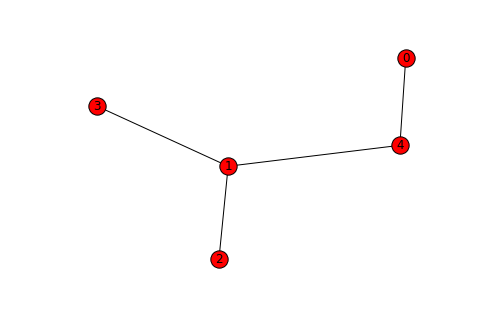
\includegraphics[width=\textwidth]{graph.png}
        \caption{A gull}
        \label{fig:gull}
    \end{subfigure}
     \begin{subfigure}[b]{0.4\textwidth}
        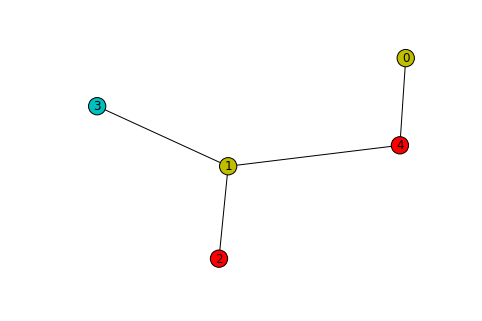
\includegraphics[width=\textwidth]{figures/colored.png}
        \caption{A gull coloured}
        \label{fig:gull}
    \end{subfigure}
\end{figure}[]



%%%%%%%%%%%%%%%%

\newpage
%\begin{multicols}{2}


%%%%%%%%%%%%%%%%%%%%%%%%%%%%%%%%%%%%%%%
\section{Implementing an Eigensolver's algorithm}
%%%%%%%%%%%%%%%%%%%%%%%%%%%%%%%%%%%%%%%


%%%%%%%%%%%%%%%%%%%%%%%%%%%%%%%%%%%%%%%%%%%
\subsection{Eigensolver's Algorithm with pyQuil}
%%%%%%%%%%%%%%%%%%%%%%%%%%%%%%%%%%%%%%%%%%%

Loading...

\newpage
%%%%%%%%%%%%%%%%%%%%%%%%%%%%%
\subsection{Eigensolver Algorithm in QISKit}
%%%%%%%%%%%%%%%%%%%%%%%%%%%%%
Applications that can use the five-qubit register include simulation of quantum state evolution and computing the properties of a ground state of the system. These applications are useful for quantum chemistry and solid state physics, where understanding strongly-correlated fermions is of interest. QISKit ACQUA provides tools that can be used to make an eigensolver for the ground state energy of simple molecules. The ground state problem may be understood as finding the solution to $H\ket{\psi_{g}}=E_{g}\ket{\psi_{g}}$, where $H$ represents the Hamiltonian (energy operator) of the system and $\ket{g}$ and $E_{g}$ represent the ground state and its associated energy, respectively. For complex systems such as molecules, the ground state energy can be challenging to compute in a simplified way. We need ACQUA to run these sorts of simulations as its library has a number of tools that simplify the process.
QISKit ACQUA requires a number of external files to run its computation. It is recommended that these steps be taken in the route to simulating molecular ground state energies with ACQUA on QISKit. The other application is in simulating the ising model of spin chains, though we will not cover this in this section.
\begin{itemize}
    \item Download the latest version of Anaconda Navigator in Python 3.6 at: \url{https://www.anaconda.com/download/}
    \item Download the relevant QISKit files from the website: \url{https://nbviewer.jupyter.org/github/QISKit/qiskit-tutorial/blob/master/index.ipynb}
    \item Sign up for QISKit via IBM Q experience and generate an API key for your Qconfig.py file found in the downloads from the QISKit website 
    \item Use the command prompt to install with: pip install qiskit qiskit-acqua qiskit-acqua-chemistry in Anaconda
\end{itemize}
The molecule in this example will be Lithium hydride (LiH), as seen in \autoref{acqua}. The Hartree Fock method (used to determine the quantum state of a multi-particle system) is used to describe the initial state of the molecule. More detail on this method of state determination can be found in \cite{hartreefockmethod}.  
\begin{lstlisting}[language=Python,float=h!,caption={The Lithium hydride eigensolver with Hartree Fock initial state adapted from \url{https://qiskit.org/acqua/chemistry}.}, label=acqua]
from qiskit_acqua_chemistry import ACQUAChemistry
# Define the problem using the parameters in the acqua dictionary
acqua_chemistry_dict = {
'driver': {'name': 'PYSCF'}, # Psycf driver for writing molecular configuration and species
# Writes the positions of the atoms in the molecule in 3 dimensions
'PYSCF': {'atom': 'Li .0 .0 -0.8; H .0 .0 0.8', 'basis': 'sto3g'},  
# Maps Hamiltonian with parity qubit mapping and two-qubit reduction. Reduces the orbital size as well 
'operator': {'name':'hamiltonian','qubit_mapping': 'parity', 'two_qubit_reduction': True, 'freeze_core': True, 'orbital_reduction': [-3,-2]},
'algorithm': {'name':'VQE'}, # Variational quantum eigensolver
# Iterates the optimizer COBYLA 10000 times
'optimizer': {'name':'COBYLA','maxiter': 10000},
'variational_form': {'name':'UCCSD'}, 
# Hartree Fock initial state calculation
'initial_state': {'name': 'Hartree Fock'}, 
# Simulation performed on the local simulator
'backend':{'name': 'local_qasm_simulator'} 
}
solver = ACQUAChemistry()
result = solver.run(acqua_chemistry_dict)
print(result['energy']) # Prints the result of the calculation for the ground state energy
\end{lstlisting}
Constrained optimisation by linear approximation (COBYLA) is the numerical optimisation, among possible others, which is used in this example. The maximum number of iterations can be altered to suit the example along with the options to print convergence trends and termination tolerance. The backend can be changed to ibmqx4 for other examples by using an API token and experiment credits on IBM Q experience. You can compare results between the two backend options to see how well ibmqx4 compares to your classical simulation. (Another example could be added after this where there are additional elements to code by the user, perhaps an exercise on this would be helpful)
\newpage

%%%%%%%%%%%%%%%%%%%%%%%%%%%%%%%%%%%%%%%%%%%
\subsection{Eigensolver's Algorithm with Project Q?}
%%%%%%%%%%%%%%%%%%%%%%%%%%%%%%%%%%%%%%%%%%%


%%%%%%%%%%%%% Old Deusch algm
\begin{comment}
\begin{multicols}{2}
%%%%%%%%%%%%%%%%%%%%%%%%%%%%%%%%


%%%%%%%%%%%%%%%%%%%%%%%%%%%%%%%%
\subsection{Deutsch's Algorithm}
%%%%%%%%%%%%%%%%%%%%%%%%%%%%%%%%

%%%%%%%%%%%%%%%%
\begin{tcolorbox}[standard jigsaw,
    opacityback=0,  % this works only in combination with the key "standard jigsaw"
    boxrule=0.5pt]
    {\bf Deutsch's Algorithm}
    \tcbline
    Given a function $f:\{0,1\}^2\rightarrow \{0,1\}$ promised to be either balanced or constant. We initialise the system in the state $\ket{00}$, we need to implement the gates $H^{\otimes 2}$ and then $U_f$ and then $H^{\otimes 2}$ and then perform a measurement in the computational basis.
\end{tcolorbox}
%%%%%%%%%%%%%%%

%%%%%%%%%%%%%%%%%
\begin{lstlisting}[language=Python,caption={Deutsch's algorithm implemented in Python only},label={lst:DApython},frame=single] 
import numpy as np
# State initialisation
state0=np.array([[1],[0],[0],[0]]) 
# Gate Implementation
H=(1/np.sqrt(2))*np.array([[1,1],[1,-1]]) 
state1=np.dot(np.kron(H,H),state0)        
U=np.array([[-1,0,0,0],
            [0,1,0,0],
            [0,0,-1,0],
            [0,0,0,1]])
state2=np.dot(U,state1)
state3=np.dot(np.kron(H,H),state2)
# Measurement: defining basis
ket0=np.array([[1],[0]])
ket1=np.array([[0],[1]])
ket00=np.kron(ket0,ket0)
ket01=np.kron(ket0,ket1)
ket10=np.kron(ket1,ket0)
ket11=np.kron(ket1,ket1)
# Measurement: projectors P00,P01,P10,P11
P00=np.dot(ket00,ket00.T)
P01=np.dot(ket01,ket01.T)
P10=np.dot(ket10,ket10.T)
P11=np.dot(ket11,ket11.T)
# Probability of obtaining: 00,01,10,11
prob00=np.trace(np.dot(P00,np.dot(state3,np.conj(state3).T)))
prob01=np.trace(np.dot(P01,np.dot(state3,np.conj(state3).T)))
prob10=np.trace(np.dot(P10,np.dot(state3,np.conj(state3).T)))
prob11=np.trace(np.dot(P11,np.dot(state3,np.conj(state3).T)))
print(prob00,prob01,prob10,prob11)
\end{lstlisting}
%%%%%%%%%%%%%%%%
\columnbreak

Now implementing this with pyQuil. We first need to learn how to add our own gates.

%%%%%%%%%%%%%%%%%
\begin{lstlisting}[language=Python]
# Defining our own gates
Ufma=np.array([[-1,0,0,0],
               [0,1,0,0],
               [0,0,-1,0],
               [0,0,0,1]]); 
p.defgate("Uf",Ufma); 
p.inst(("Uf",0,1)); 
\end{lstlisting}
%%%%%%%%%%%%%%%%

In \autoref{lst:DAqvm}

%%%%%%%%%%%%%%%%%
\begin{lstlisting}[language=Python,caption={Deutsch's algorithm with pyQuil},label={lst:DAqvm},frame=single]
import numpy as np
from pyquil.quil import Program
from pyquil.api import QVMConnection 
from pyquil.gates import X,Z,Y,H,I 
# Invoking and renaming
qvm=QVMConnection()
p=Program() 
# Gate implementation
p.inst(H(0),H(1)) 
# Assuming the given function gives
Ufma=np.array([[-1,0,0,0],
               [0,1,0,0],
               [0,0,-1,0],
               [0,0,0,1]]);
# Adding matrix as a gate               
p.defgate("Uf",Ufma); 
# Applying new gate and Hadamards
p.inst(("Uf",0,1)); 
p.inst(H(0),H(1))
# Measurements
p.measure(0,0)
p.measure(1,1) 
# Running the program
cr=[] 
results=qvm.run(p,cr,4) 
print(results)
\end{lstlisting}
%%%%%%%%%%%%%%%%

%%%%%%%%%%%%%%%%
\begin{tcolorbox}[standard jigsaw,
    opacityback=0,  % this works only in combination with the key "standard jigsaw"
    boxrule=0.5pt]
    {\bf Exercise 2: Bernstein-Vazirani Algorithm}
    \tcbline
    As in DJ with $n=3$, and given a function $f$ that is a parity function. Checking that the code indeed identifies the parity function
\end{tcolorbox}

\end{multicols}
\end{comment}
%%%%%%%%%%%%%


%%%%%%%%%%%%%% Old Rigetti code added by Ben
\begin{comment}
Rigetti has created an environment called Forest, amongst its contributions is a python library called PyQuil. With PyQuil one can simulate up to 26 qubits on the Quantum Virtual Machine (QVM). An example code from \cite{rigetti} is detailed below with comments to assist the reader:
%%%%%%%%%%%%%%%%%%%%%%%%%%%%%%%%%%%
\begin{lstlisting}[language=Python,float=h]
from pyquil.quil import Program
from pyquil.gates import H, CNOT
from pyquil.api import SyncConnection
# construct a Bell State program
p = Program()
p.inst(H(0))
p.inst(CNOT(0, 1))
# run the program on a QVM
qvm = SyncConnection()
result = qvm.wavefunction(p) 
# produces the output wavefunction of the Bell state
\end{lstlisting}
Rigetti also offers access to a 19 qubit processor they call 19Q. This API 
%%%%%%%%%%%%%%%%%%%%%%%%%%%%%%%%%%%%%%%%%%%
\begin{lstlisting}[language=Python,float=h]
import numpy as np
 
def incmatrix(genl1,genl2):
    m = len(genl1)
    n = len(genl2)
    M = None #to become the incidence matrix
    VT = np.zeros((n*m,1), int)  #dummy variable
 
    #compute the bitwise xor matrix
    M1 = bitxormatrix(genl1)
    M2 = np.triu(bitxormatrix(genl2),1) 
 
    for i in range(m-1):
        for j in range(i+1, m):
            [r,c] = np.where(M2 == M1[i,j])
            for k in range(len(r)):
                VT[(i)*n + r[k]] = 1;
                VT[(i)*n + c[k]] = 1;
                VT[(j)*n + r[k]] = 1;
                VT[(j)*n + c[k]] = 1;
 
                if M is None:
                    M = np.copy(VT)
                else:
                    M = np.concatenate((M, VT), 1)
 
                VT = np.zeros((n*m,1), int)
 
    return M
\end{lstlisting}
\end{comment}
%%%%%%%%%%%%%